\documentclass[12pt, twoside]{article}
\usepackage[letterpaper, margin=1in, headsep=0.5in]{geometry}
\usepackage[english]{babel}
\usepackage[utf8]{inputenc}
\usepackage{amsmath}
\usepackage{amsfonts}
\usepackage{amssymb}
\usepackage{tikz}
%\usetikzlibrary{quotes, angles}

\usepackage{graphicx}
\usepackage{enumitem}
\usepackage{multicol}

\usepackage{fancyhdr}
\pagestyle{fancy}
\fancyhf{}
\renewcommand{\headrulewidth}{0pt} % disable the underline of the header

\usepackage{setspace}
%\linespread{1.75}

%\fancyhead[RE]{\thepage}
\fancyhead[R]{\thepage \\ Name: \hspace{3cm}}
\fancyhead[L]{BECA / Dr. Huson / 12.1 IB Math SL\\* 29 March 2019}

\begin{document}
\subsubsection*{7-9 Homework: Mixed Calculus - without calculator \hfill [58 marks]}
 \begin{enumerate}

%\subsubsection*{You may NOT use a calculator on these problems \hfill [52 marks]}

\setstretch{1.2}

\item 12M.1.sl.TZ1.3 \hfill [6 marks]\\
Let $f(x)=e^{6x}$.
\begin{enumerate}
  \item Write down $f'(x)$ \hfill [1]
  \item The tangent to the graph of $f$ at the point $P(0,b)$ has gradient $m$.  \hfill [4]
  \begin{enumerate}
    \item Show that $m=6$.
    \item Find $b$.
  \end{enumerate}
  \item Hence, write down the equation of this tangent. \hfill [1]
\end{enumerate}

\item 09M.1.sl.TZ1.3 \hfill [6 marks]\\
Let $f(x)=e^{x} \cos x$. Find the gradient of the normal to the curve of $f$ at $x= \pi$.

\item 13M.1.sl.TZ1.3 \hfill [7 marks]\\
Consider $f(x)=x^2 \sin x$.
\begin{enumerate}
  \item Find $f'(x)$. \hfill [4]
  \item Find the gradient of the curve of $f$ at $x= \frac{\pi}{2}$. \hfill [3]
\end{enumerate}

\item 12N.1.sl.TZ0.4 \hfill [6 marks]\\
Part of the graph of $f(x)= ax^3-6x^2$ is shown below.
  \begin{center}
    \begin{tikzpicture}[scale=3]
      \draw [thick, ->] (-0.8,0) -- (1.8,0) node [below] {$x$};
      \draw [thick, ->] (0,-1.5) -- (0,0.5) node [left] {$y$};
      \draw[thick, domain=-0.40:1.25] plot[samples=100](\x, {5*(\x)^3 - 6*(\x)^2});
      \draw[dashed] (1,0)node[above]{$1$} --(1,-1) node[right]{P};
      \node at (1,-1) {\textbullet};
    \end{tikzpicture}
  \end{center}

  The point $P$ lies on the graph of $f$. At $P$, $x=1$.
  \begin{enumerate}
    \item Find $f'(x)$. \hfill [2]
    \item The graph of $f$ has a gradient of 3 at the point $P$. Find the value of $a$. \hfill [4]
  \end{enumerate}

\newpage
\item Let $f(x)=x^2$. \hfill [6 marks]
  \begin{enumerate}
    \item Find $\int_1^2 (f(x))^2 \,\mathrm{d}x$ \hfill [4]
    \item The following diagram shows part of the graph of $f$.
      \begin{center}
        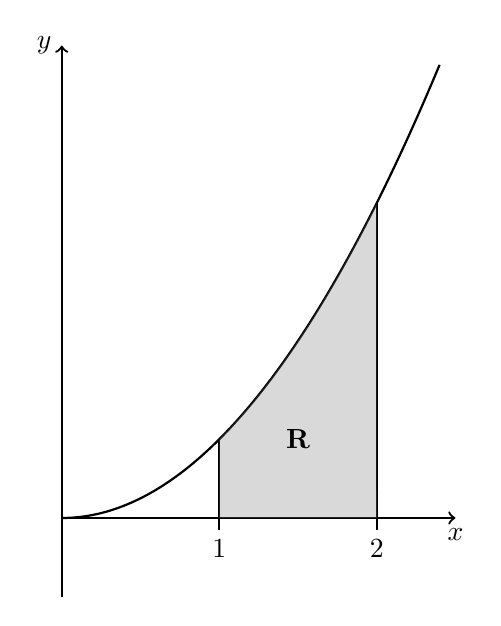
\begin{tikzpicture}[xscale=2,yscale=1]
          \draw [thick, ->] (0,0) -- (2.5,0) node [below] {$x$};
          \draw [thick, ->] (0,-1) -- (0,6) node [left] {$y$};
          \draw[thick, domain=0:2.4] plot[samples=100](\x, {(\x)^2});
          \draw[thick] (1, -.15)node[below]{$1$} --(1,1);
          \draw[thick] (2, -.15)node[below]{$2$} --(2,4);
          \fill[gray,opacity=.3] (1,0)--plot[domain=1:2](\x, {\x*\x})--(2,0);
          \draw (1.5,1) node {$\mathbf{R}$};
        \end{tikzpicture}
      \end{center}
    The shaded region $R$ is enclosed by the graph of $f$, the $x$-axis, and the lines $x=1$ and $x=2$.\\
    Find the volume of the solid formed when $R$ is revolved $360^\circ$ about the $x$-axis.  \hfill [2]
  \end{enumerate}

\item 13N.1.sl.TZ0.4 \hfill [6 marks]\\
  Consider a function $f(x)$ such that $\int_2^5 f(x) \,\mathrm{d}x
  =10$.
  \begin{enumerate}
    \item Find $\int_2^5 3f(x) \,\mathrm{d}x$. \hfill [2]
    \item Find $\int_2^5 (f(x)+12) \,\mathrm{d}x$. \hfill [4]
  \end{enumerate}

\newpage
\item 17M.1.sl.TZ1.6 \hfill [6 marks]\\
The following diagram shows the graph of $f'$, the derivative of $f$.
  \begin{center}
    \begin{tikzpicture}[x=0.8cm, y=0.4cm]
      \draw [thick, ->] (-4,0) -- (10.5,0) node [below right] {$x$};
      \draw [thick, ->] (0,-12) -- (0,9) node [left] {$y$};
      \foreach \x in {-4,..., 10}
      \draw[shift={(\x,0)},color=black] (0pt,-3pt) -- (0pt,0pt) node[below=4pt]  {$\x$};
      \foreach \y in {-12,-10,...,8}
      \draw[shift={(0,\y)},color=black] (-3pt,0pt) -- (0pt,0pt) node[left=3pt]  {$\y$};

      \draw[thick, domain=-2:9] plot[samples=100](\x, {-0.104*(\x+0.9118)*(\x-6)^2});
      \draw [fill] (1.39,-5.09) circle [radius=0.05cm] node[below] {$A$};
      \draw [fill] (4,-2.01) circle [radius=0.05cm] node[below right]{$(4,-2)$};
      \draw [fill] (6,0) circle [radius=0.05cm] node[above] {$B$};
           %\draw[dashed] (1,0)node[above]{$1$} --(1,-1) node[right]{P};
    \end{tikzpicture}
  \end{center}

  The graph of $f'$ has a local minimum at $A$, a local maximum at $B$ and passes through $(4,2)$. The point $P(4,3)$ lies on the graph of the function, $f$.
  \begin{enumerate}
    \item Write down the gradient of the curve of $f$ at $P$.\hfill  [1]
    \item Find the equation of the normal to the curve of $f$ at $P$.\hfill  [3]
    \item Determine the concavity of the graph of $f$ when $4<x<5$ \textbf{and} justify your answer.\hfill  [2]
  \end{enumerate}

  \item 16M.1.sl.TZ1.10 \hfill [15 marks]\\
  Let $f(x)=\sqrt{4x+5}$, for $x \geq -1.25$.
  \begin{enumerate}
    \item Find $f'(1)$. \hfill [4]
    \item Consider another function $g$. Let $R$ be a point on the graph of $g$. The $x$-coordinate of $R$ is 1. The equation of the tangent to the graph at $R$ is  $y=3x+6$.\\
    Write down $g'(1)$. \hfill [2]
    \item Find $g(1)$. \hfill [2]
    \item Let $h(x)=f(x) \times g(x)$. Find the equation of the tangent to the graph of $h$ at the point where $x=1$. \hfill [7]
  \end{enumerate}


\end{enumerate}
\end{document}
